\chapter{Estado del arte}

En este capítulo se analizan los fundamentos teóricos y las tecnologías existentes que conforman la base de este proyecto. Se revisan las principales bases de datos clínicas abiertas, las arquitecturas de software para la gestión de datos sanitarios, las herramientas de visualización interactiva y las aplicaciones de la Inteligencia Artificial en el ámbito clínico.

\section{El Movimiento hacia la Ciencia Abierta en la Investigación Médica}

En las últimas décadas se ha consolidado un movimiento hacia los datos clínicos abiertos, promoviendo la disponibilidad de bases de datos sanitarias para la comunidad investigadora. La idea de ciencia abierta sostiene que la libre disponibilidad de datos y códigos favorece la transparencia, la reproducibilidad y la colaboración en la investigación biomédica \cite{Lvovs2025_balancing}. Sin embargo, históricamente los datos clínicos han estado protegidos en archivos hospitalarios, difíciles de acceder por razones legales, éticas y técnicas. En respuesta, iniciativas académicas y gubernamentales han impulsado la creación de conjuntos de datos clínicos de acceso abierto, debidamente anonimizados, que permiten a investigadores de todo el mundo analizar información real de pacientes sin vulnerar la privacidad. Estos recursos han transformado la investigación médica al reducir barreras de acceso y fomentar prácticas reproducibles en análisis de datos sanitarios

\newpage
Los datos clínicos se pueden clasificar en cuatro grandes modalidades complementarias:


(i) \emph{Señales fisiológicas de alta frecuencia.} Series temporales de ECG, presión arterial invasiva, fotopletismografía o EEG. Podemos destacar la clásica MIT-BIH Arrhythmia Database (1980), patrón de referencia para algoritmos de ECG \cite{Impact_MIT-BIH}; el MIMIC Waveform Database, que enlaza miles de horas de señales con los datos clínicos de MIMIC \cite{Moody2022_MIMICIVWaveform}; y HiRID, con 712 variables registradas cada dos minutos en más de 30 000 estancias UCI \cite{Faltys2021HiRID}.

(ii) \emph{Imágenes médicas con anotaciones diagnósticas.}  Abarcan radiografías, TC, RM, PET e incluso histopatología digital, cada una acompañada de etiquetas o informes de hallazgo.  Las bases más usadas en radiología son ChestXray14 y CheXpert, ambas con cientos de miles de radiografías torácicas etiquetadas para patologías pulmonares \cite{irvin2019chexpertlargechestradiograph}, y MIMIC-CXR por parte de la familia MIMIC \cite{Johnson2019_MIMICCXR}.  En oncología destacan las colecciones TCGA/TCIA \cite{TCGA,Clark2013_TCIA}, y en neuroimagen la iniciativa ADNI \cite{Petersen2010_ADNI}.  Estos recursos posibilitan evaluar modelos de visión computacional con criterios homogéneos.

(iii) \emph{Texto clínico desidentificado.}  Incluye notas de evolución, informes radiológicos, resúmenes de alta, entre otros.  Representa alrededor del 80 \% de la información clínica, pero su liberación es más compleja por contener PHI (Protected Health Information).  Los desafíos i2b2/n2c2, pioneros al proveer corpora anonimizados, constituyen la plataforma estándar para comparar sistemas de procesamiento del lenguaje natural médico \cite{n2c2}.  El ecosistema MIMIC también complementa este dominio con millones de notas clínicas \cite{Johnson2023_MIMICIVNote}. 

(iv) \emph{Datos estructurados de historias clínicas electrónicas (EHR).}  Comprenden tablas con demografía, diagnósticos (ICD-9/10), procedimientos, resultados de laboratorio, medicación y constantes vitales.  Son la base de estudios epidemiológicos y de la construcción de modelos pronósticos.  Entre los conjuntos abiertos más influyentes figuran NHANES \cite{NHANES}, UK Biobank \cite{Sudlow2015_UKBiobank}, eICU \cite{Pollard2018} y, sobre todo, la serie MIMIC en la que se enfoca este trabajo.

Desde 1999 PhysioNet \cite{PhysioNet_paper} estableció un marco seguro y reproducible para compartir todo tipo de registros hospitalarios.  Bajo ese paraguas nació el ecosistema MIMIC: la primera versión (1996) contenía 90 pacientes UCI \cite{Moody1996_MIMIC}; MIMIC-II (2011) multiplicó tamaño y variables al extraer directamente de los sistemas clínicos \cite{Saeed2011_MIMICII}; MIMIC-III (2015) superó los 40 000 pacientes y se convirtió en la referencia mundial \cite{MIMICIII_paper}; MIMIC-IV \cite{MIMICIV_paper} amplía y moderniza el conjunto.  Esta trayectoria demuestra cómo los EHR han pasado a ser un recurso científico global, permitiendo investigar la fisiopatología crítica con una profundidad antes impensable.

\newpage
En conjunto, el panorama de datos clínicos abiertos ofrece múltiples alternativas, pero MIMIC-IV destaca como la más idónea para este trabajo: combina un gran volumen de datos reciente, buena documentación, y módulos complementarios. Sobre esta base, el proyecto diseñará una plataforma que haga de este conjunto de datos una fuente accesible de conocimiento, alineada con los principios de ciencia abierta que han guiado todo este repaso bibliográfico.


\section{Tecnologías para la Gestión y Almacenamiento de Datos Sanitarios}




En el plano tecnológico, la forma de almacenar y consultar la información marca las posibilidades reales de análisis. De forma general, los sistemas de gestión de bases de datos se dividen en dos grandes familias: relacionales y no relacionales. Las del primer grupo organizan la información en tablas de filas y columnas conectadas por claves y se consultan con SQL, siendo las más usadas MySQL, PostgreSQL, Oracle y SQL Server.  Las no relacionales, llamadas NoSQL, almacenan los datos como documentos, pares clave-valor, columnas o grafos y permiten esquemas flexibles y escalado horizontal; las más populares son MongoDB y Couchbase en la categoría de documentos, Cassandra en column-family, Redis en clave-valor y Neo4j en grafos \cite{DBEngines2025}.

En el ámbito sanitario la mayoría de los sistemas de historia clínica electrónica se ha construido sobre gestores relacionales porque los registros se modelan de forma natural en tablas normalizadas y el lenguaje SQL facilita auditoría y trazabilidad.  Sin embargo, los hospitales también generan notas de texto libre, señales continuas, imágenes y estructuras jerárquicas como los recursos FHIR en JSON; ello ha impulsado el uso de bases documentales y de grafos, que aceptan datos heterogéneos y simplifican la ingesta sin migraciones de esquema cada vez que aparece un nuevo campo \cite{GAMAL2021103670,MongoFHIR}.

A pesar de que MIMIC-IV se distribuye en un esquema relacional, para este proyecto cargaremos el conjunto en MongoDB. Este modelo documental nos permite agrupar los datos que se deseen en un único documento anidado, elimina la necesidad de combinar una veintena de tablas con uniones complejas y responde con menor latencia a las búsquedas interactivas que planteará el usuario desde la interfaz web.  Además, nos ofrece flexibilidad y escalabilidad si en el futuro se desea incorporar señales o imágenes, de modo que se adapta mejor a la naturaleza exploratoria y multimodal de nuestra aplicación.


\section{Arquitecturas de Software y el Stack Tecnológico Web}

La evolución del desarrollo de software ha experimentado una transformación radical desde las aplicaciones de escritorio tradicionales hacia ecosistemas web distribuidos. En los años 90, la Web se caracterizaba por páginas estáticas servidas directamente desde servidores, pero la creciente demanda de interactividad y funcionalidad dinámica impulsó el desarrollo de tecnologías como CGI, PHP y posteriormente frameworks más sofisticados \cite{Ritesh2023_WebEvolution}. Esta evolución culminó en las aplicaciones web contemporáneas, que se fundamentan en la arquitectura cliente-servidor, donde el frontend ejecutado en el navegador del usuario se comunica con un backend que procesa la lógica y gestiona el acceso a los datos \cite{Nyabuto2024_ClientServer}. Esta separación de responsabilidades permite que cada componente evolucione independientemente, facilita el mantenimiento del código y posibilita la escalabilidad según las necesidades específicas de cada capa. En el contexto de aplicaciones de análisis de datos como la que nos ocupa, esta arquitectura resulta especialmente ventajosa al permitir que el procesamiento computacionalmente intensivo se realice en el servidor mientras el cliente se centra en la presentación interactiva de los resultados.

En cuanto a las tecnologías de servidor, existe un amplio abanico de alternativas consolidadas, cada una con fortalezas específicas según el contexto de aplicación. Node.js con frameworks como Express o Fastify permite utilizar JavaScript en el servidor, facilitando el desarrollo full-stack y ofreciendo excelente rendimiento para aplicaciones I/O intensivas. Python, con opciones como Django, Flask y FastAPI, destaca en proyectos que requieren análisis de datos o integración con librerías científicas \cite{Castro2023_PythonDataScience}. Java con Spring Boot sigue siendo una opción robusta para aplicaciones empresariales de gran escala, mientras que lenguajes como Go y Rust están ganando adopción por su rendimiento superior en sistemas distribuidos. En el contexto de este proyecto, donde el procesamiento de datos biomédicos y la futura integración de modelos de inteligencia artificial son requisitos centrales, se ha optado por FastAPI con Python, aprovechando tanto su ecosistema maduro para análisis de datos como su capacidad para generar APIs modernas y eficientes.

Por otro lado, las tecnologías frontend han experimentado una evolución significativa desde las aplicaciones de página única (SPA) hacia enfoques más sofisticados que combinan diferentes estrategias de renderizado. Los frameworks principales \cite{Swacha2023_WebFrameworks} incluyen React, que ofrece un ecosistema maduro y flexible basado en componentes; Vue.js, conocido por su curva de aprendizaje suave y documentación excelente; y Angular, que proporciona un framework completo con opiniones definidas para aplicaciones empresariales. Paralelamente, han surgido meta-frameworks como Next.js, Nuxt.js y SvelteKit que extienden estos frameworks base con capacidades de renderizado del lado del servidor (SSR), generación de sitios estáticos (SSG) y optimizaciones automáticas. Para este proyecto se ha seleccionado Next.js sobre React, desplegado en Vercel, una combinación que permite aprovechar tanto el renderizado híbrido para optimizar el rendimiento del análisis y visualización de datos.

\begin{figure}[htbp]
\centering
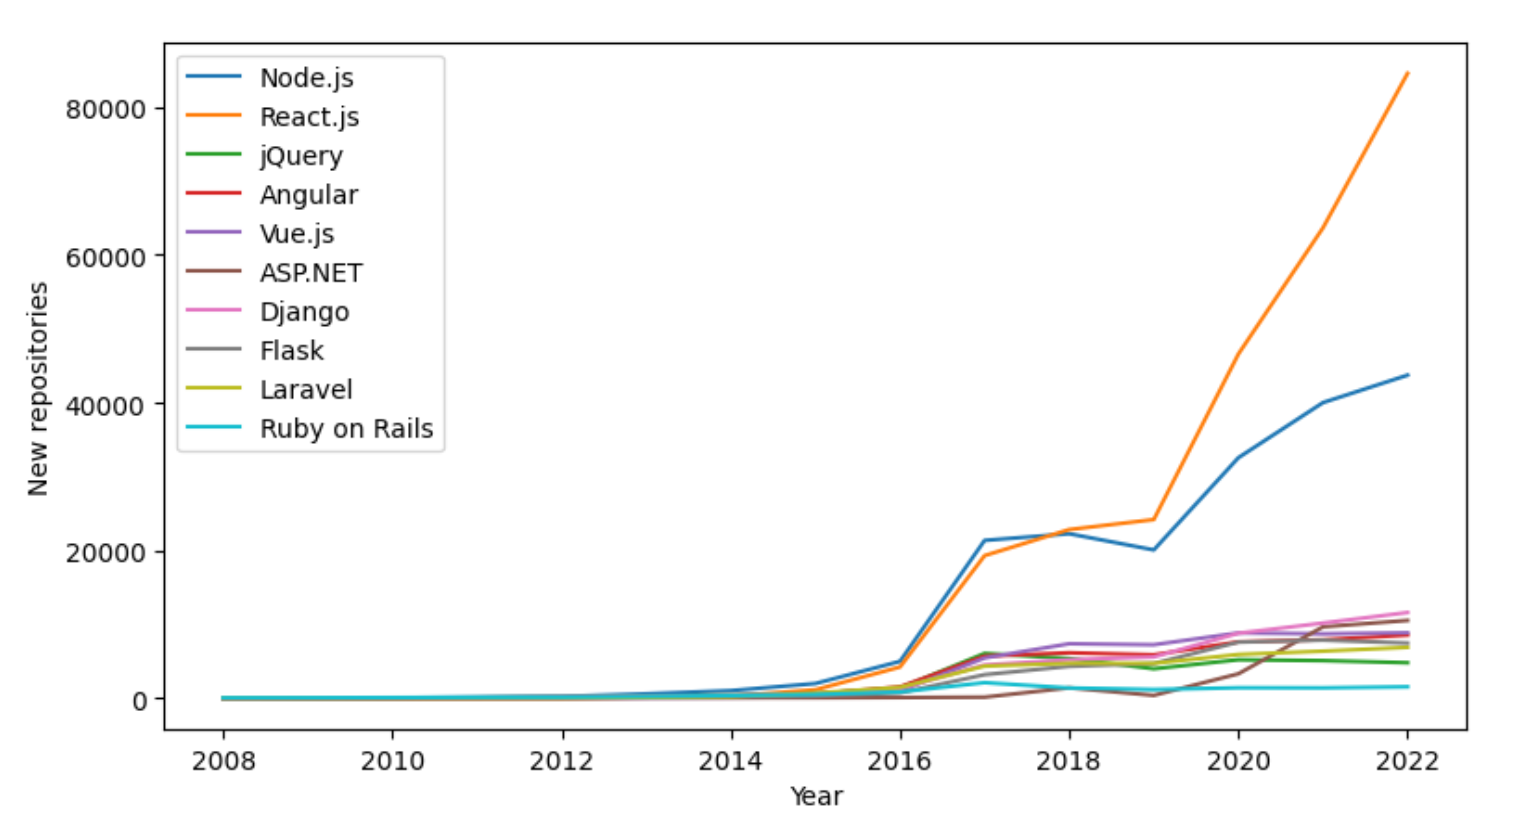
\includegraphics[width=\textwidth]{imagenes/grafica_frameworks.png}
\caption{Evolución de la popularidad de frameworks web según el número de repositorios creados anualmente en GitHub \cite{Swacha2023_WebFrameworks}.}
\label{fig:frameworks_github}
\end{figure}



\section{Herramientas y Técnicas de Visualización Interactiva de Datos}

Para la visualización de datos en aplicaciones web existen principalmente dos tipos de herramientas: plataformas de business intelligence (Tableau, Power BI, Metabase) y librerías de programación para desarrolladores. Entre las librerías más utilizadas destacan D3.js, Chart.js, Plotly.js, ECharts, Recharts, Nivo, Vega-Lite y Observable Plot \cite{Monterail2024_JSViz}. En el contexto de este proyecto, se ha optado por Observable Plot para gráficos sencillos debido a su API intuitiva y soluciones preestablecidas que aceleran el desarrollo, complementándolo con Nivo para visualizaciones más complejas que Observable Plot pero sin necesitar recurrir a D3.js, y reservando D3.js para visualizaciones altamente personalizadas que requieren máximo control granular, manteniendo así un enfoque progresivo en complejidad que maximiza tanto la rapidez de implementación como la flexibilidad de diseño.

\section{Aplicaciones de Inteligencia Artificial en el Análisis Clínico}

En la última década se ha producido un auge sin precedentes de la inteligencia artificial en el ámbito médico, impulsado por los avances en aprendizaje profundo y la creciente disponibilidad de datos clínicos masivos. Grandes bases de datos abiertas han permitido a los investigadores entrenar modelos con mejor rendimiento en tareas complejas, demostrando que los algoritmos de machine learning pueden superar a los métodos tradicionales en aplicaciones como predicción de mortalidad o duración de estancia hospitalaria \cite{Nature2022_MIMICDeepLearning}. En este contexto emergen dos enfoques principales: los modelos predictivos de riesgo clínico basados en datos estructurados, y los asistentes conversacionales que utilizan técnicas de procesamiento del lenguaje natural para democratizar el acceso a la información médica.

Un uso destacado de la IA en medicina es la construcción de modelos predictivos que anticipen riesgos clínicos a partir de datos tabulares de los pacientes. Históricamente se han utilizado métodos clásicos de aprendizaje automático como la regresión logística o los bosques aleatorios por su interpretabilidad y buen desempeño en datos clínicos estructurados. Sin embargo, en los últimos años los modelos de aprendizaje profundo han ganado protagonismo al demostrar mayor rendimiento en estas tareas \cite{Frontiers2022_MLPrediction}. Las aplicaciones más comunes incluyen predicción de mortalidad hospitalaria, detección temprana de sepsis, estimación de duración de estancia y evaluación de riesgo de readmisión \cite{Nature2023_SepsisML}. Estos modelos se entrenan sobre características derivadas de datos demográficos, signos vitales, resultados de laboratorio y registros de medicación, permitiendo generar alertas tempranas o indicadores de riesgo que pueden integrarse directamente en las visualizaciones de datos clínicos.

Paralelamente, la irrupción de los grandes modelos de lenguaje ha abierto nuevas posibilidades para crear interfaces conversacionales que permitan a usuarios no técnicos interactuar con bases de datos complejas mediante lenguaje natural. Estos sistemas han experimentado una adopción masiva sin precedentes, con herramientas como ChatGPT superando los 100 millones de usuarios en solo un mes \cite{AcademyHealth2025_LLM}. En el dominio sanitario, esta tecnología está dando lugar a asistentes conversacionales médicos como ChatEHR de Stanford, que permite a los profesionales conversar con historiales electrónicos utilizando preguntas en lenguaje cotidiano \cite{Stanford2025_ChatEHR}. Estos sistemas combinan técnicas de procesamiento del lenguaje natural con arquitecturas de generación aumentada por recuperación (RAG) \cite{RAGSurvey2023} para traducir preguntas en lenguaje natural a consultas estructuradas, representando una oportunidad significativa para democratizar el acceso a bases de datos complejas como MIMIC-IV.

La integración de ambos enfoques en plataformas de visualización de datos representa el futuro hacia el que se dirige este proyecto. Los modelos predictivos pueden generar indicadores de riesgo que se muestren directamente en los gráficos interactivos, mientras que los asistentes conversacionales pueden facilitar tanto la exploración de datos como la interpretación de patrones complejos. El desarrollo de protocolos como Model Context Protocol (MCP) \cite{AnthropicMCP2024,MCPIntro2024} está proporcionando nuevas arquitecturas para conectar directamente los asistentes de IA con bases de datos, ofreciendo una alternativa más flexible que RAG para consultas complejas sobre datos estructurados. Esta convergencia entre visualización, predicción e interacción conversacional promete democratizar el análisis de datos clínicos y acelerar el descubrimiento de conocimiento médico.